\documentclass[11pt]{article}
\usepackage{geometry, titlesec}
\usepackage[parfill]{parskip}
\usepackage[italicdiff]{physics}
\usepackage{amsfonts, amsthm}
\usepackage[cm]{fullpage}
\usepackage{fancyhdr}
\usepackage{enumitem}
\usepackage{xcolor, soul}
\usepackage{graphicx}
\usepackage[export]{adjustbox}
\usepackage{siunitx}
%\allowdisplaybreaks

\renewcommand{\thesubsection}{\thesection.\alph{subsection}}
\setenumerate[1]{label={(\alph*)}}

\makeatletter
\renewcommand*\env@cases[1][1.2]{%
  \let\@ifnextchar\new@ifnextchar
  \left\lbrace
  \def\arraystretch{#1}%
  \array{@{}l@{\quad}l@{}}%
}
\makeatother
 
\renewcommand{\footrulewidth}{.2pt}
%\setlist[enumerate]{leftmargin=*}
\pagestyle{fancy}
\fancyhf{}
\lhead{Physics 132-B}
\chead{\textbf{Discussion 6 Solutions}}
\rhead{A--De Discussion}
\setlength{\headheight}{11pt}
\setlength{\headsep}{11pt}
\setlength{\footskip}{24pt}
\lfoot{\today}
\rfoot{\thepage}

\titleformat{\subsection}[runin]{\normalfont\large\bfseries}{\thesubsection}{1em}{}
\newcommand{\refeq}[1]{(\ref{#1})}

\newcommand{\beq}{\begin{equation*}}
\newcommand{\eeq}{\end{equation*}}

\newcommand{\beqn}{\begin{equation}}
\newcommand{\eeqn}{\end{equation}}

\newcommand{\blg}{\begin{align*}}
\newcommand{\elg}{\end{align*}}


\newenvironment{statement}
{
%    \color{gray}
    \ignorespaces
}
{
%    \smallskip
}

\newenvironment{problem}
{
    \color{darkgray}
    \ignorespaces
}

\newenvironment{solution}
{
    \paragraph{Solution.}
    \ignorespaces
}
{
    \bigskip
}

\renewcommand{\vec}[1]{\mathbf{#1}}


\begin{document}
	


\paragraph{Question 24.2}
\begin{problem}
	Suppose several different parallel-plate capacitors are charged up by a constant-voltage source.  Thinking of the actual movement and position of the charges on an atomic level, why does it make sense that the capacitances are proportional to the areas of the plates?  Why does it makes sense that the capacitances are \emph{inversely} proportional to the distance between the plates?
\end{problem}

\begin{solution}
	When we close a circuit with a battery and a capacitor, electrons flow through the wires from the battery to one plate of the capacitor.  They cannot easily ``jump'' onto the next plate because the dielectric material separating the plates is not a perfect conductor.  But they are still being pushed away from the voltage source, so they will go as far as they possibly can, which is the surface of the capacitor plate.  The larger the surface area $A$, the more electrons can gather on it, and so the greater the magnitude of charge $Q$ that accumulates on the plate's surface.  Capacitance is proportional to this charge: $C = Q/V \propto A/V$.
	
	The buildup of charge on the first capacitor plate sets up an electric field $\vb{E}$ between the two plates.  This electric field has an associated electric potential $V$, which can be found by $V = \int_a^b \vb{E} \cdot \dd{\vb{l}} = E d$, where $d$ is the distance between the plates.  So the potential difference across the plates is proportional to $d$.  The capacitance is inversely proportional to this potential difference: $C = Q/V \propto Q/d$.
\end{solution}

\vfill


\newcommand{\eps}{\epsilon}

\paragraph{Question 24.20}
\begin{problem}
	A conductor is an extreme case of a dielectric, since if an electric field is applied to a conductor, charges are free to move within the conductor to set up ``induced charges.''  What is the dielectric constant $K$ of a perfect conductor?  Explain your reasoning.
\end{problem}

\begin{solution}
	The dielectric constant $K$ is closely related to a perhaps more useful quantity, which is the permittivity $\eps$ of the dielectric:
	\beqn \tag{24.17} \label{24.17}
		\eps = K \eps_0.
	\eeqn
	We know that an electric field in free space is proportional to $1 / (4\pi\eps_0)$.  Likewise, the electric field in a dielectric material is proportional to $1 / (4\pi\eps)$.  But we know the electric field inside a perfect conductor is zero!  So if it is proportional to $1 / (4\pi\eps)$, we need $\eps \to \infty$, which means $K \to \infty$ by Eq.~\refeq{24.17}.
\end{solution}

\vfill


\newcommand{\Vab}{V_{ab}}

\paragraph{Question 25.17}
\begin{problem}
	The energy that can be extracted from a storage battery is always less than the energy that goes into is while it is being charged.  Why?
\end{problem}

\begin{solution}
	A real-life battery always has some internal resistance.  This means that some of the energy we put into the battery while charging it is dissipated as heat.  That is, we have already lost some of the energy that we put into the battery, because it wasn't stored in the first place.  When we discharge the battery, we have to deal with the internal resistance again.  Some of the energy that we try to extract is also dissipated as heat.  So energy is lost going in, and going out!
\end{solution}

\vfill

\clearpage



\begin{minipage}[l]{0.75\textwidth}
\paragraph{Question 25.14}
\begin{problem}
	A light bulb glows because it has resistance.  The brightness of a light bulb increases with the electrical power dissipated in the bulb. \medskip
	\begin{enumerate}
		\item In the circuit shown in \textbf{Fig.~Q25.14(a)}, the two bulbs $A$ and $B$ are identical.  Compared to bulb $A$, does bulb $B$ glow more brightly, just as brightly, or less brightly?  Explain your reasoning. \medskip
		\item Bulb $B$ is removed from the circuit and the circuit is completed as shown in \textbf{Fig.~Q25.14(b)}.  Compared to the brightness of bulb $A$ in \textbf{Fig.~Q25.14(a)}, does bulb $A$ now glow more brightly, just as brightly, or less brightly?  Explain your reasoning.
	\end{enumerate}
\end{problem}
\end{minipage}%
\hspace{0.05\textwidth}%
\begin{minipage}{0.2\textwidth}
\center 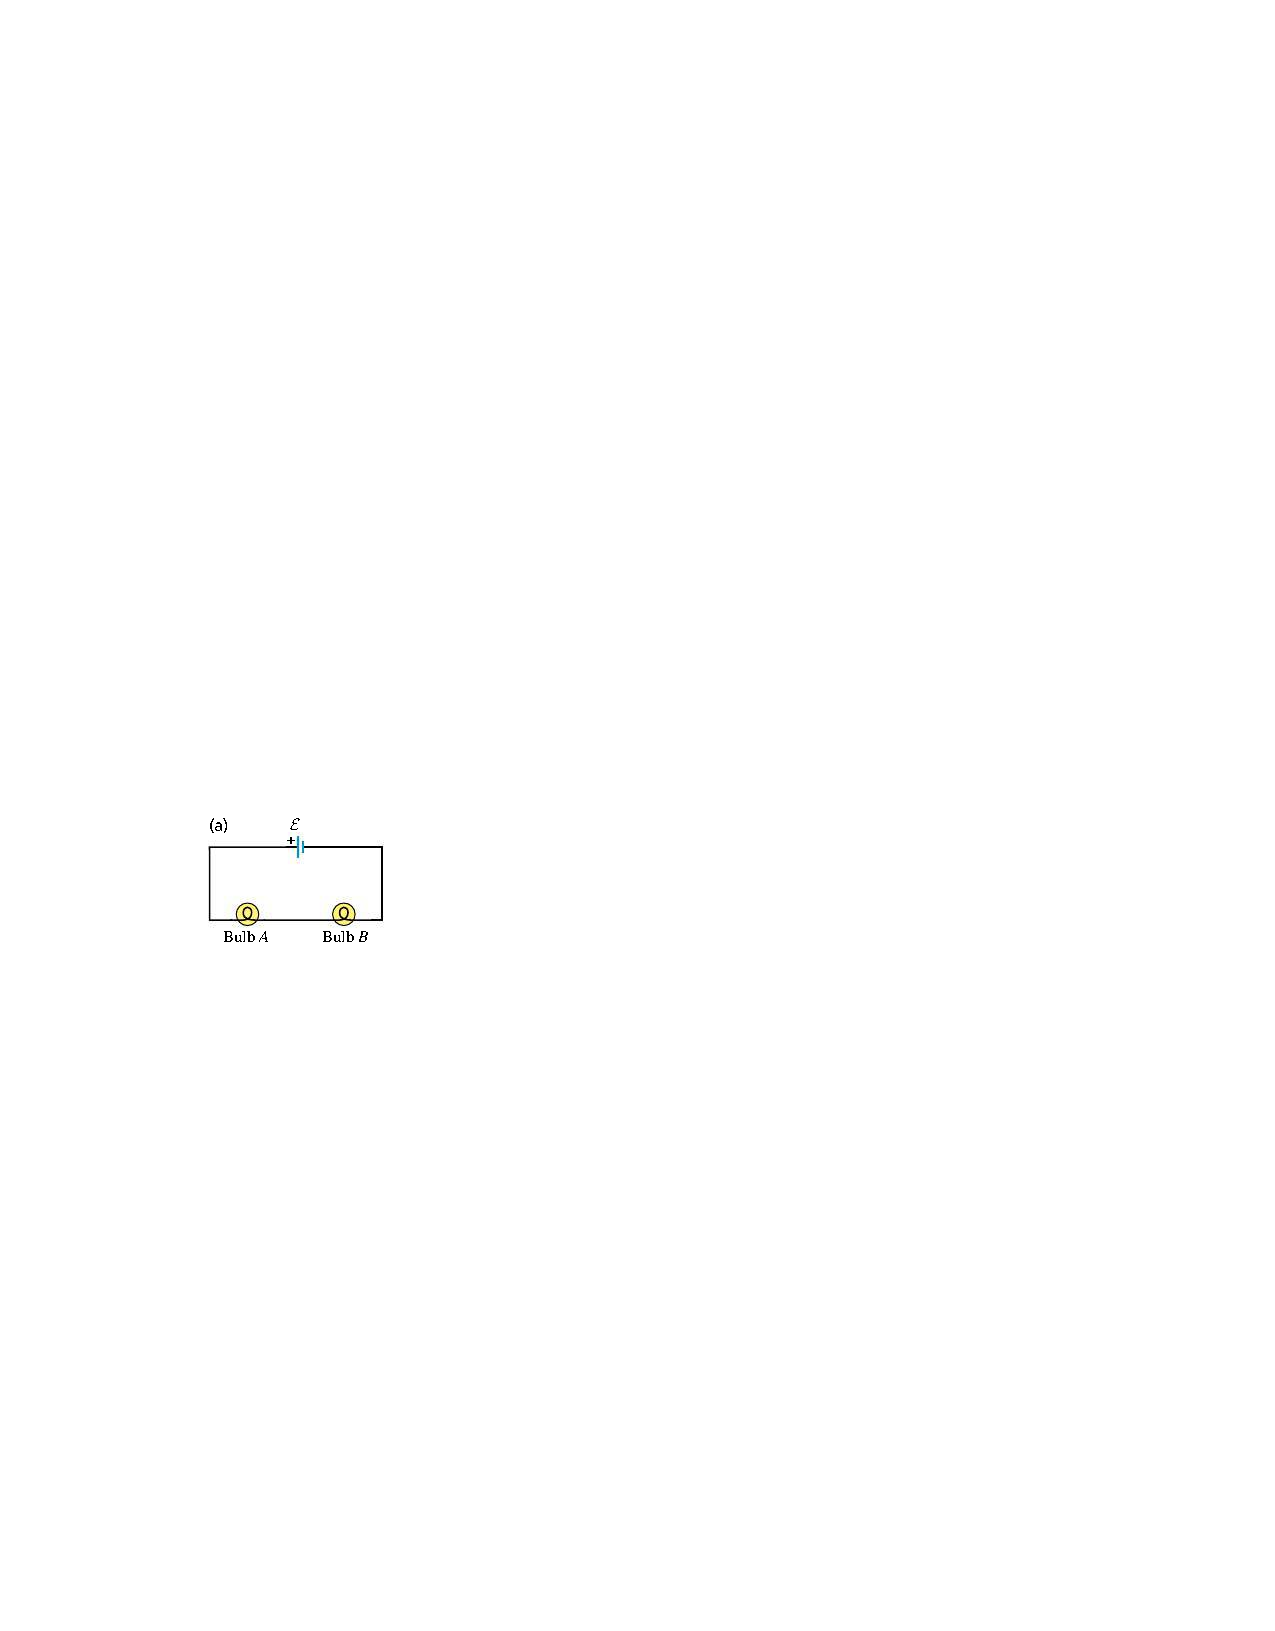
\includegraphics{Q25-14a} \\
\center 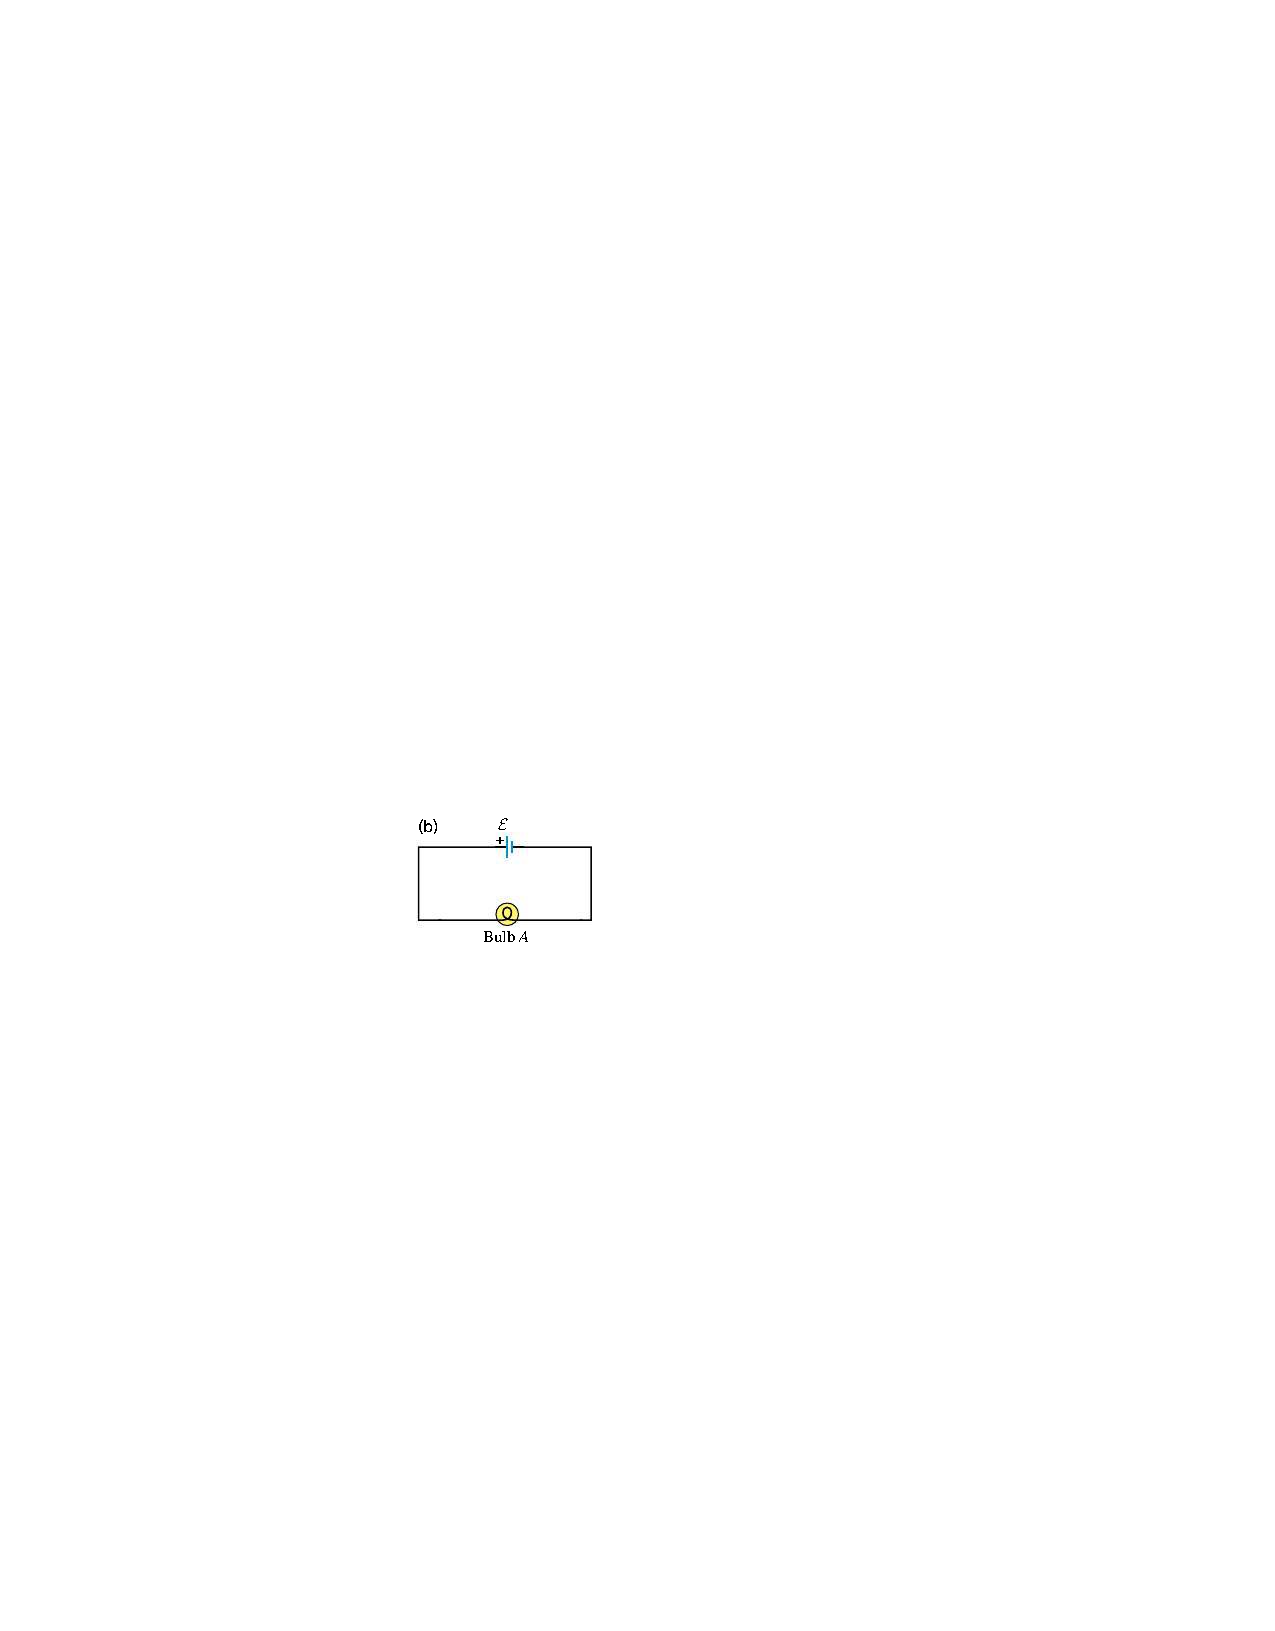
\includegraphics{Q25-14b}
\center \textbf{Figure Q25.14}
\end{minipage}

\begin{solution}
	\begin{enumerate}
		\item The bulbs are connected in series, so the current $I$ through them is the same.  We are told they are identical, so they have the same resistance $R$.  The power delivered to each bulb is then identical: $P = I^2 R$.  So bulb $B$ glows just as brightly as bulb $A$.
		\item The equivalent resistance is smaller in circuit (b) because bulb $B$ is not connected in series.  The current $I$ through bulb $A$ in circuit (b) is therefore greater than in circuit (a), so bulb $A$ now glows more brightly.
	\end{enumerate}
\end{solution}

\vfill

\newcommand{\Req}{R_\text{eq}}
\newcommand{\Rtot}{R_\text{tot}}

\begin{minipage}[l]{0.7\textwidth}
\paragraph{Question 26.9}
\begin{problem}
	A light bulb is connected in the circuit shown in \textbf{Fig.~Q26.9}.  If we close the switch $S$, does the bulb's brightness increase, decrease, or stay the same?  Why?
\end{problem}
\end{minipage}%
\hspace{0.05\textwidth}%
\begin{minipage}{0.25\textwidth}
\center 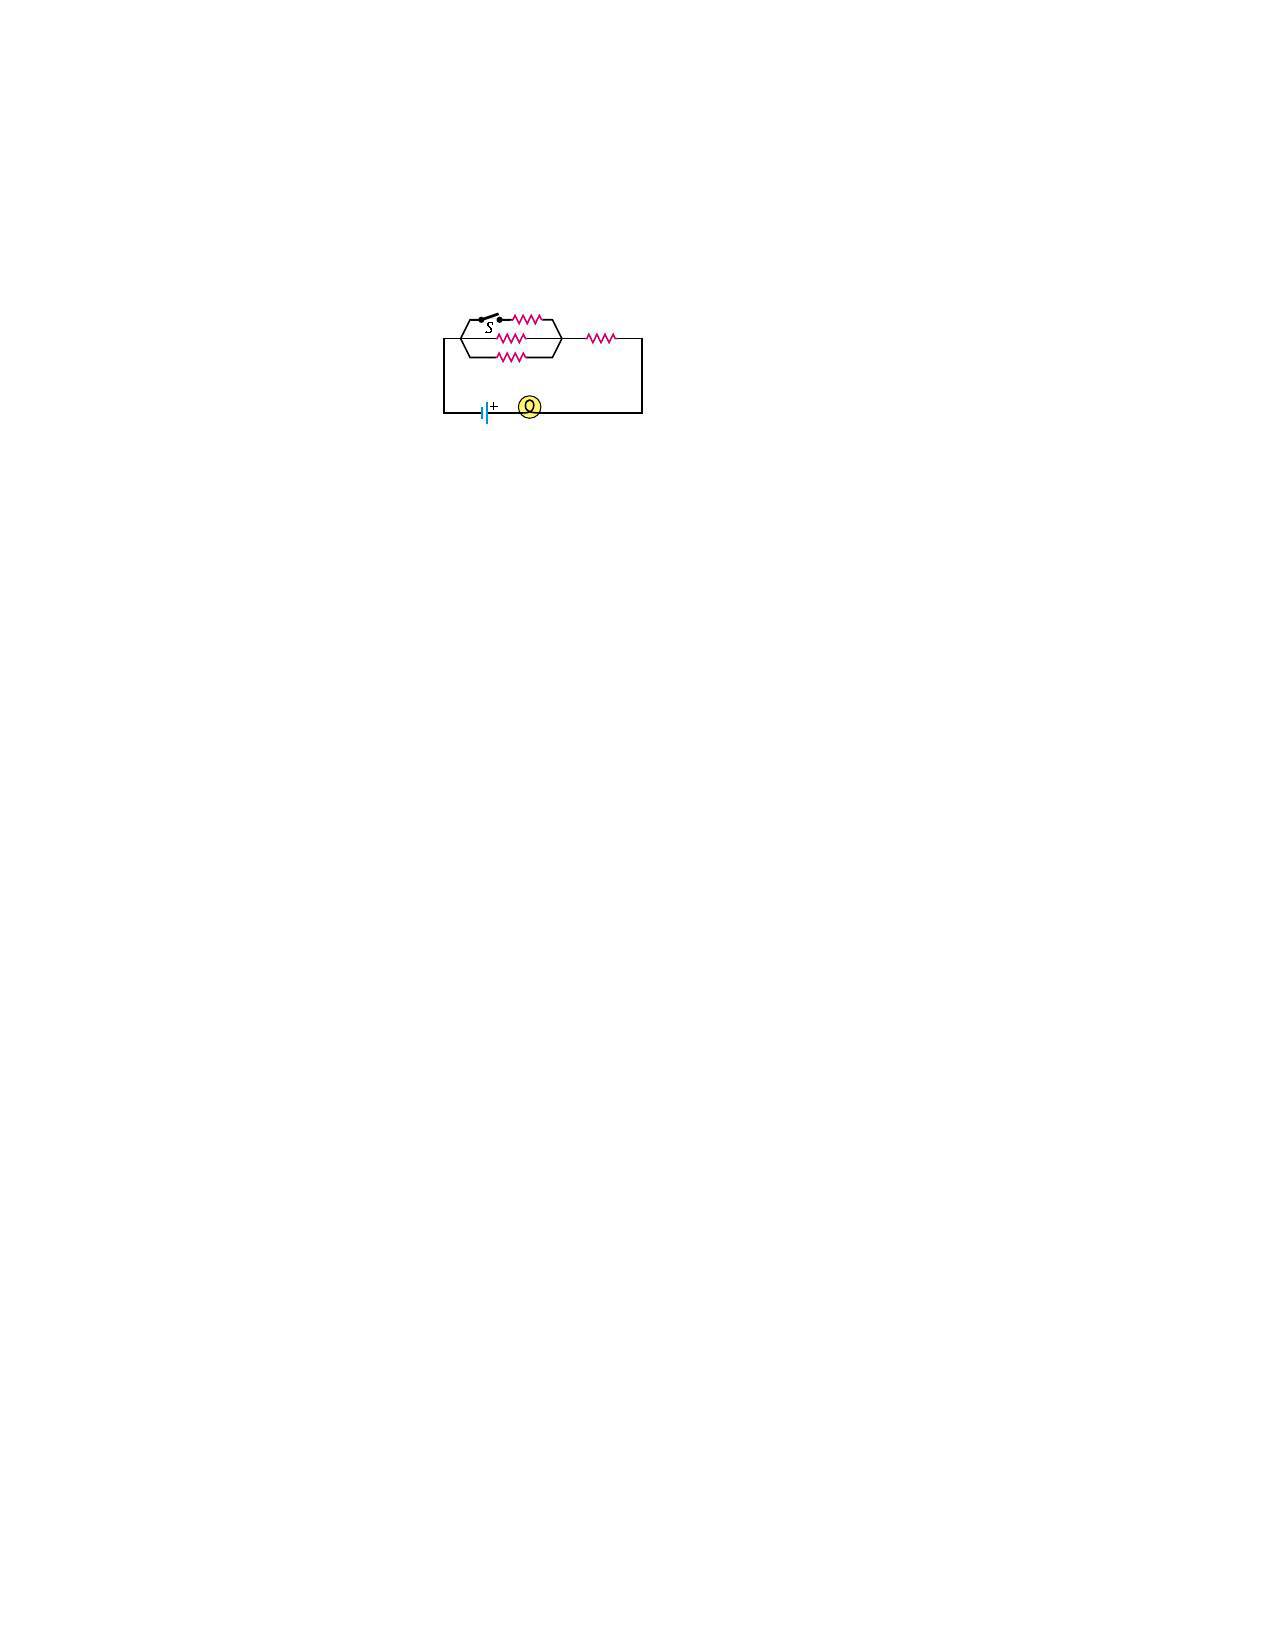
\includegraphics{Q26-9}
\center \textbf{Figure Q26.9}
\end{minipage}

\begin{solution}
	For the purposes of this problem, we can assume all of the resistors have the same resistance $R$.  Before $S$ is closed, the equivalant resistance of the two resistors connected in parallel is given by
	\beq
		\frac{1}{\Req} = \frac{1}{R} + \frac{1}{R} = \frac{2}{R}
		\implies
		\Req = \frac{R}{2},
	\eeq
	so the total resistance in the loop (excluding the bulb) is
	\beq
		\Rtot = R + \frac{R}{2} = \frac{3}{2} R.
	\eeq
	
	After $S$ is closed, the equivalent resistance of all three resistors is given by
		\beq
		\frac{1}{\Req^S} = \frac{1}{R} + \frac{1}{R} + \frac{1}{R} = \frac{3}{R}
		\implies
		\Req^S = \frac{R}{3},
	\eeq
	so the total resistance in the loop (excluding the bulb) is
	\beq
		\Rtot^S = R + \frac{R}{3} = \frac{4}{3} R,
	\eeq
	which is \emph{less} than is was before we closed the switch.  So, by similar reasoning as in \textbf{Question 25.14}, the bulb's brightness increases.
\end{solution}

%\vfill

\clearpage

\newcommand{\Ceq}{C_\text{eq}}
\newcommand{\ssa}{^{(\text{a})}}
\newcommand{\ssb}{^{(\text{b})}}

\begin{minipage}[l]{0.5\textwidth}
\paragraph{Question 26.18}
\begin{problem}
	Will the capacitors in the circuits shown in \textbf{Fig.~Q26.18} charge at the same rate when the switch $S$ is closed?  If not, in which circuit will the capacitors charge more rapidly?  Explain.
\end{problem}
\end{minipage}%
\hspace{0.05\textwidth}%
\begin{minipage}{0.45\textwidth}
\center {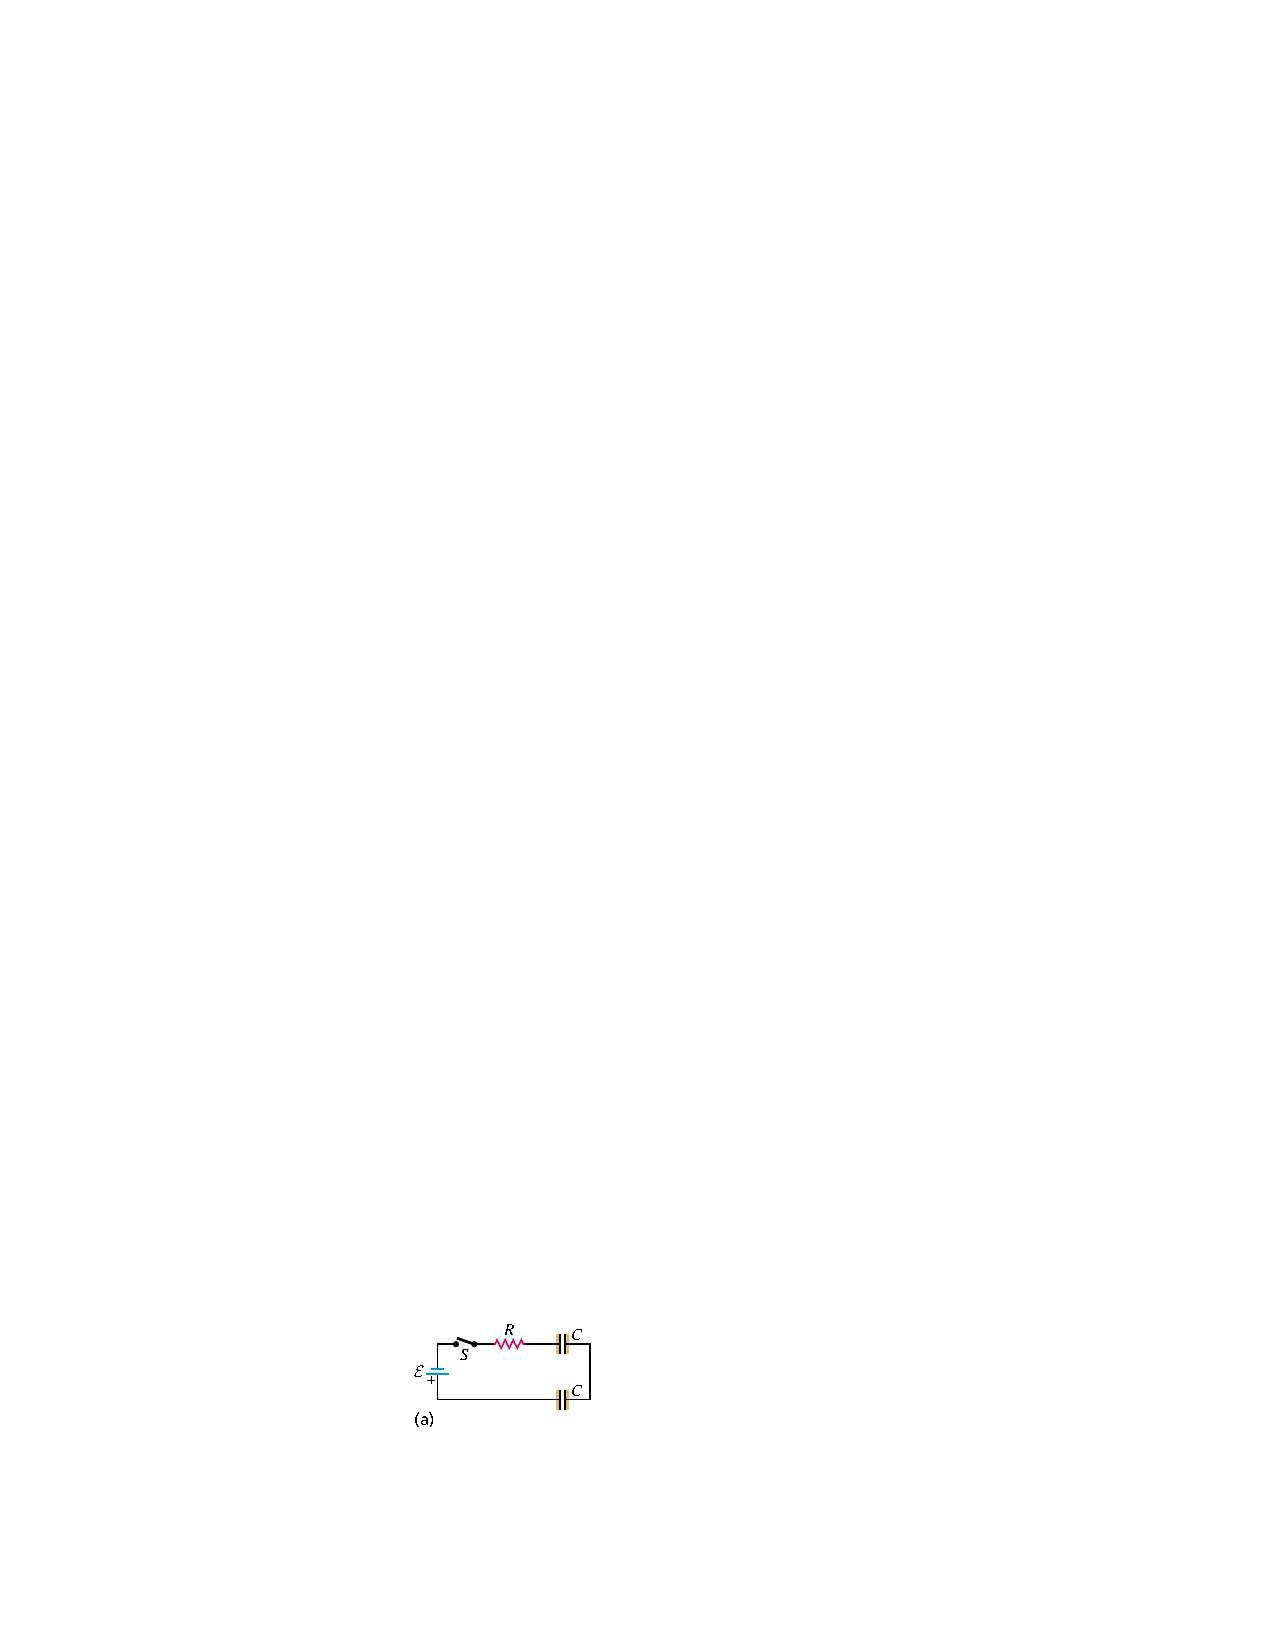
\includegraphics{Q26-18a}
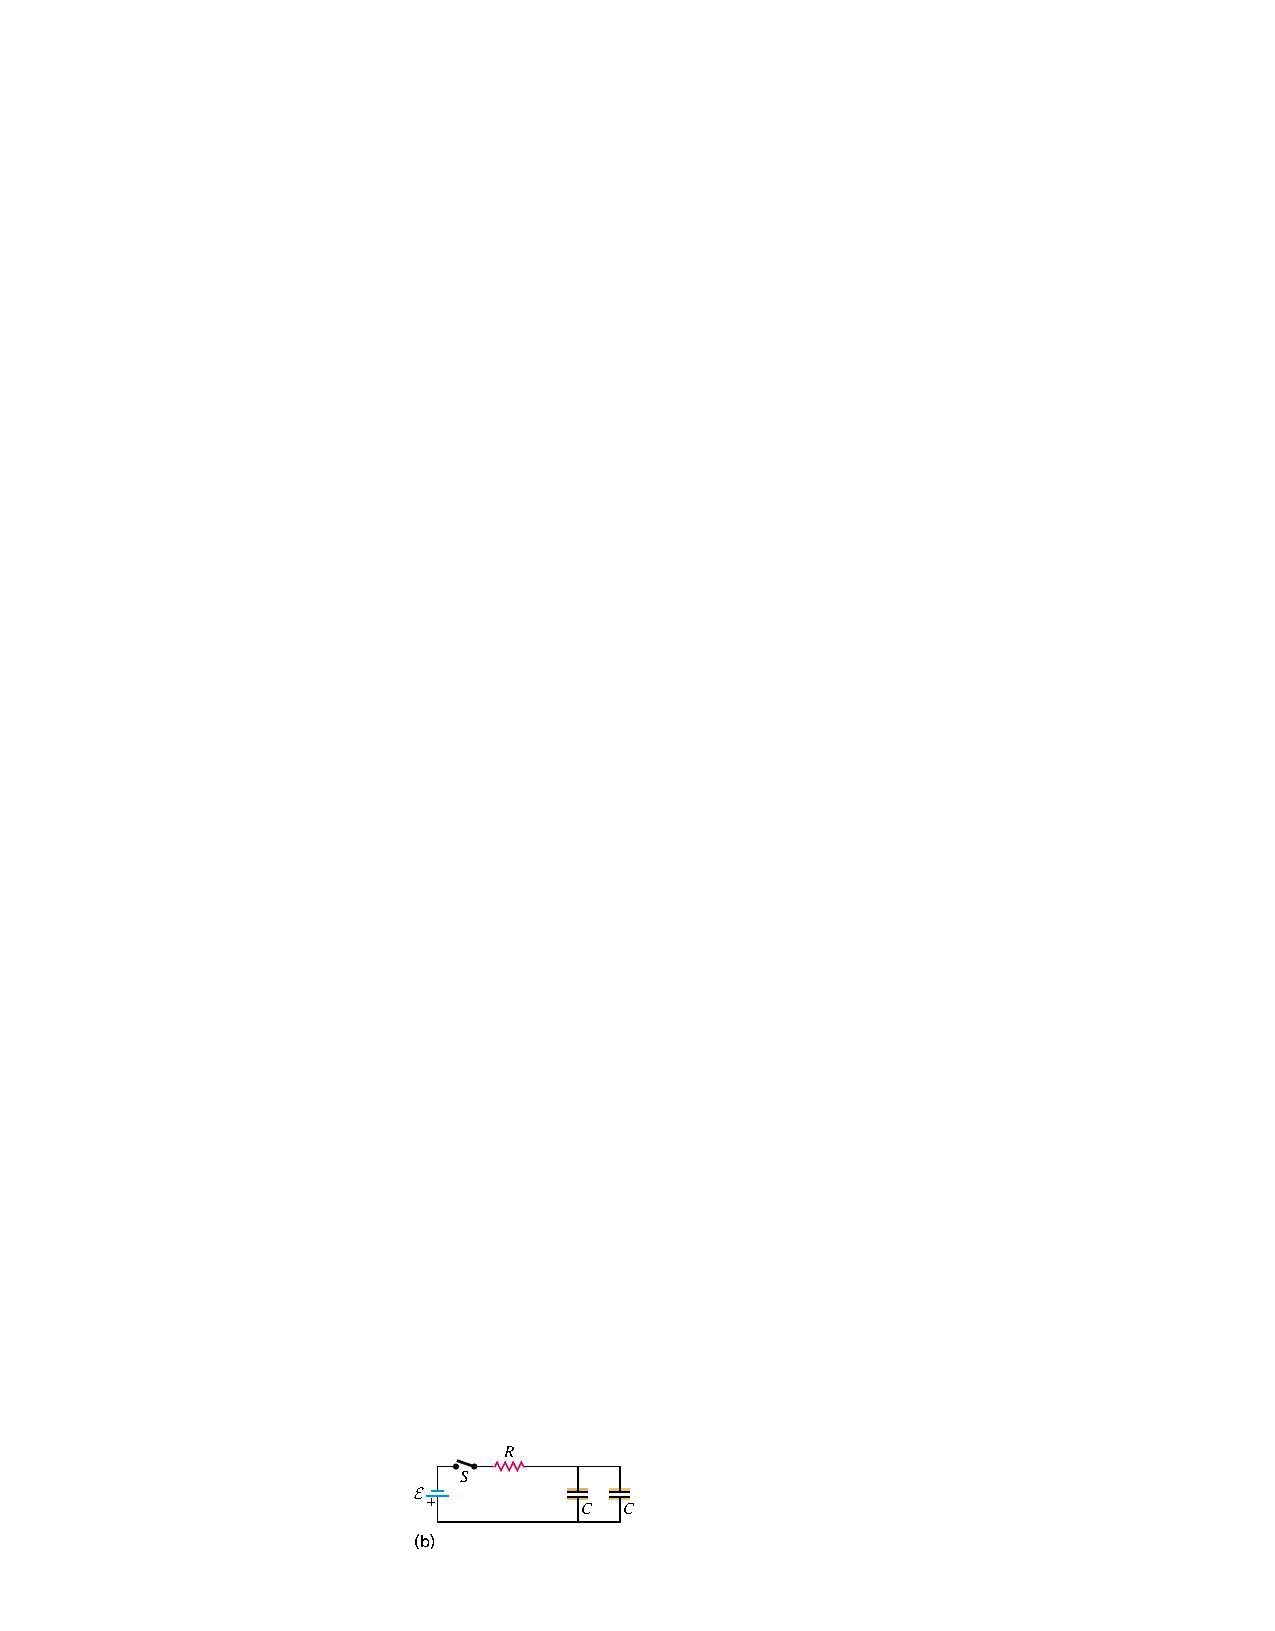
\includegraphics{Q26-18b}}
\center \textbf{Figure Q26.18}
\end{minipage}

\begin{solution}
	The time it takes to charge a capacitor in an $RC$ circuit is proportional to the time constant $\tau$, defined
	\beqn \label{26.14}
		\tau = R C,
	\eeqn
	where $R$ is the resistance of the resistor connected in series and $C$ is the capacitor's capacitance.
	
	For the purposes of this problem, we can assume both capacitors have the same capacitance $C$.  In circuit (a), the capacitors are connected in series so their equivalent capacitance is given by
	\beq
		\frac{1}{\Ceq\ssa} = \frac{1}{C} + \frac{1}{C} = \frac{2}{C}
		\implies
		\Ceq\ssa = \frac{C}{2},
	\eeq
	which gives the time constant
	\beq
		\tau\ssa = \frac{R C}{2}.
	\eeq
	
	In circuit (b), the capacitors are connected in parallel, so their equivalent capacitance is
	\beq
		\Ceq\ssb = C + C = 2C,
	\eeq
	which gives the time constant
	\beq
		\tau\ssb = 2 C R.
	\eeq
	
	The time constants are not the same, so the capacitors will not charge at the same rate in both circuits.  The time constant for (a) is smaller, so the capacitors in circuit (a) will charge more rapidly.
\end{solution}

\vfill

\end{document}